\section{Jakarta}\label{sec:jakarta}
Jakarta is a 7-qubit machine, with a Falcon r5.11H processor. 

Why 7 qubit is our Hamiltonian has only tree states? 
The other four states can be used as ancilla qubits in the decomposition and/or to reduce noise in noise reduction techniques. State Tomography at the end will be done only on qubit 1,3,5 (and you can't change which qubits will me measured) while other qubits will not be measured and so they are free to use as one like.

\paragraph{Gates}
We can use the native gates of the machine, the following set of gates are universal, therefore any gate can be implemented even without Qiskit Pulse, however there could be a significant improvement using only native gates\footnote{e.g. avoiding overlapping of errors of the native gates}. Here is the list:
   \begin{description}
    \item[\textbf{ID}: ] Identity
    \item[\textbf{CNOT}: ] CNOT Gate
    \item[\textbf{Z}: ] Z Gate
    \item[\textbf{SX}: ] Pauli-X Gate Squared
    \item[\textbf{X}: ] Pauli-X Gate
   \end{description}

In figure~\ref{fig:jakarta1} and figure~\ref{fig:jakarta2} we see the full specifications of Jakarta. Specifically in figure~\ref{fig:jakarta2} we see the various errors in the native gates. Note that those errors fluctuate quite significantly over time.

In figure~\ref{fig:cnot-error}, figure~\ref{fig:pauli-error} and figure~\ref{fig:sx-error} we see the different errors in the native gates divided per qubit. 

Initially it was attempted to exploit those different errors in order to create a decomposition that uses as less as possibile gates on qubit with high errors on those gates. However, over time, this strategy has not proved to be successful, especially for the already mentioned high fluctuation of errors during time.
    
\begin{figure}
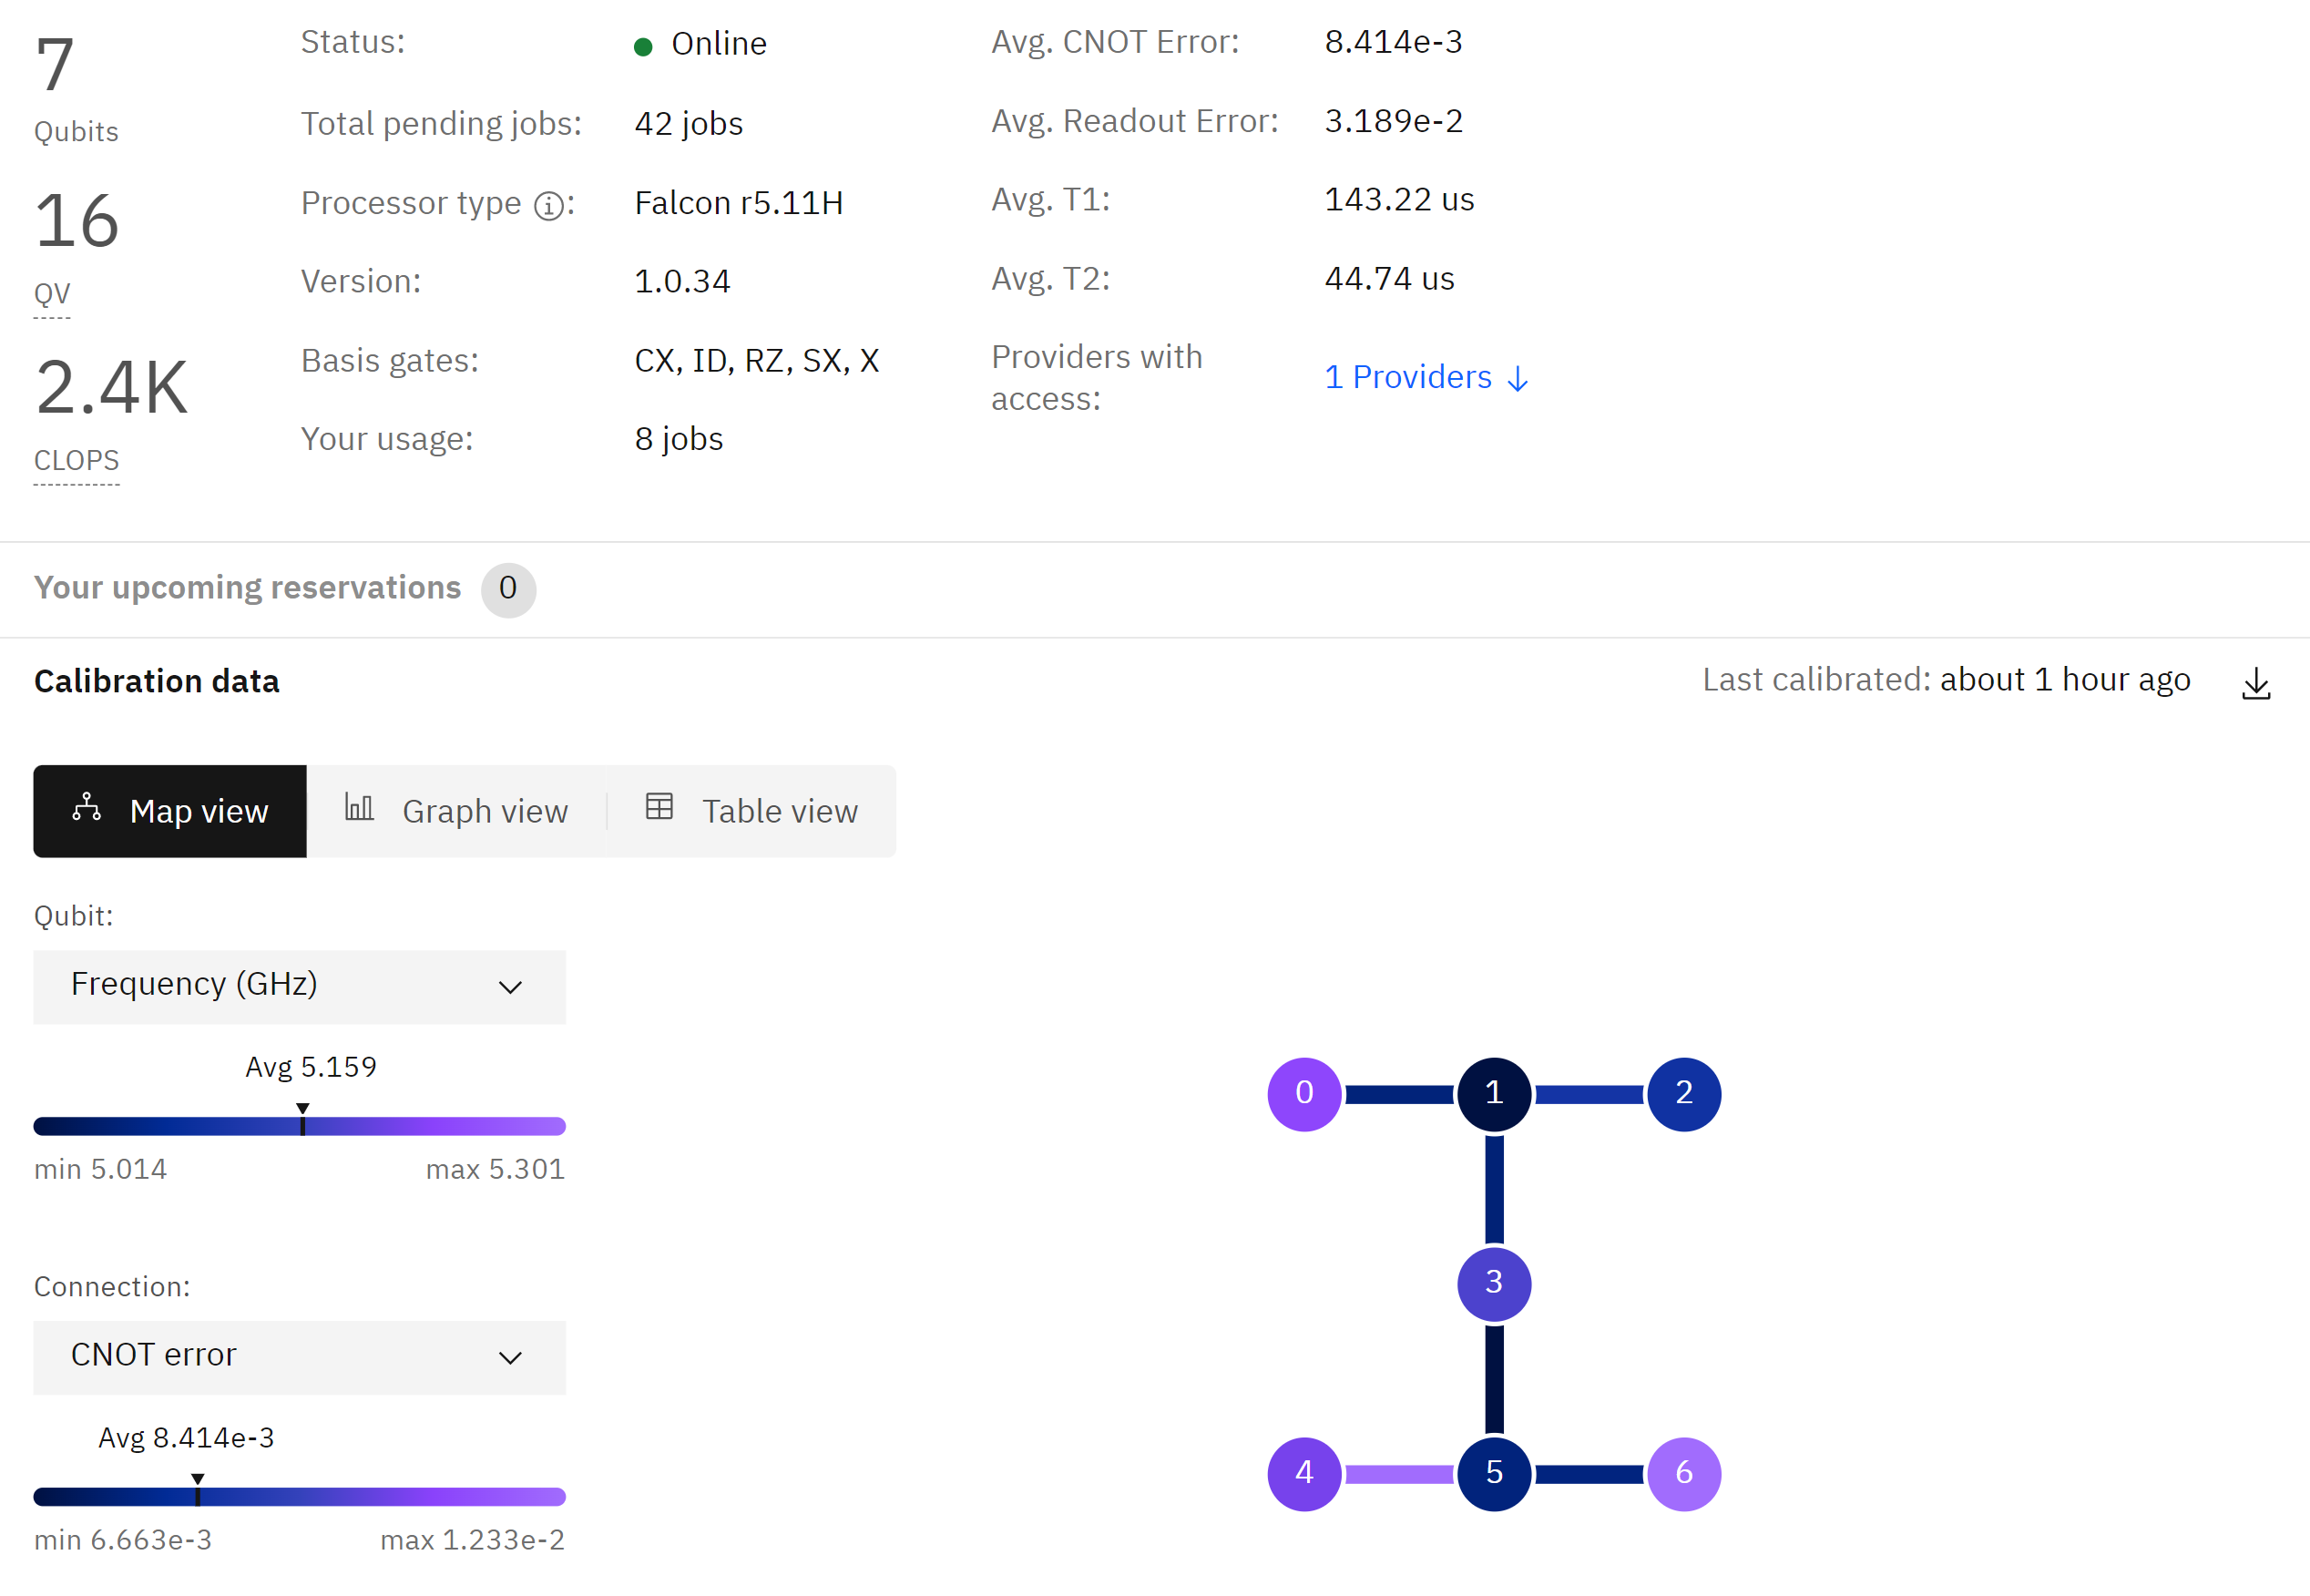
\includegraphics[width = 1.5\textwidth]{jakarta1.png}
\centering
\caption{The machine}
\label{fig:jakarta1}
\end{figure}

\begin{figure}
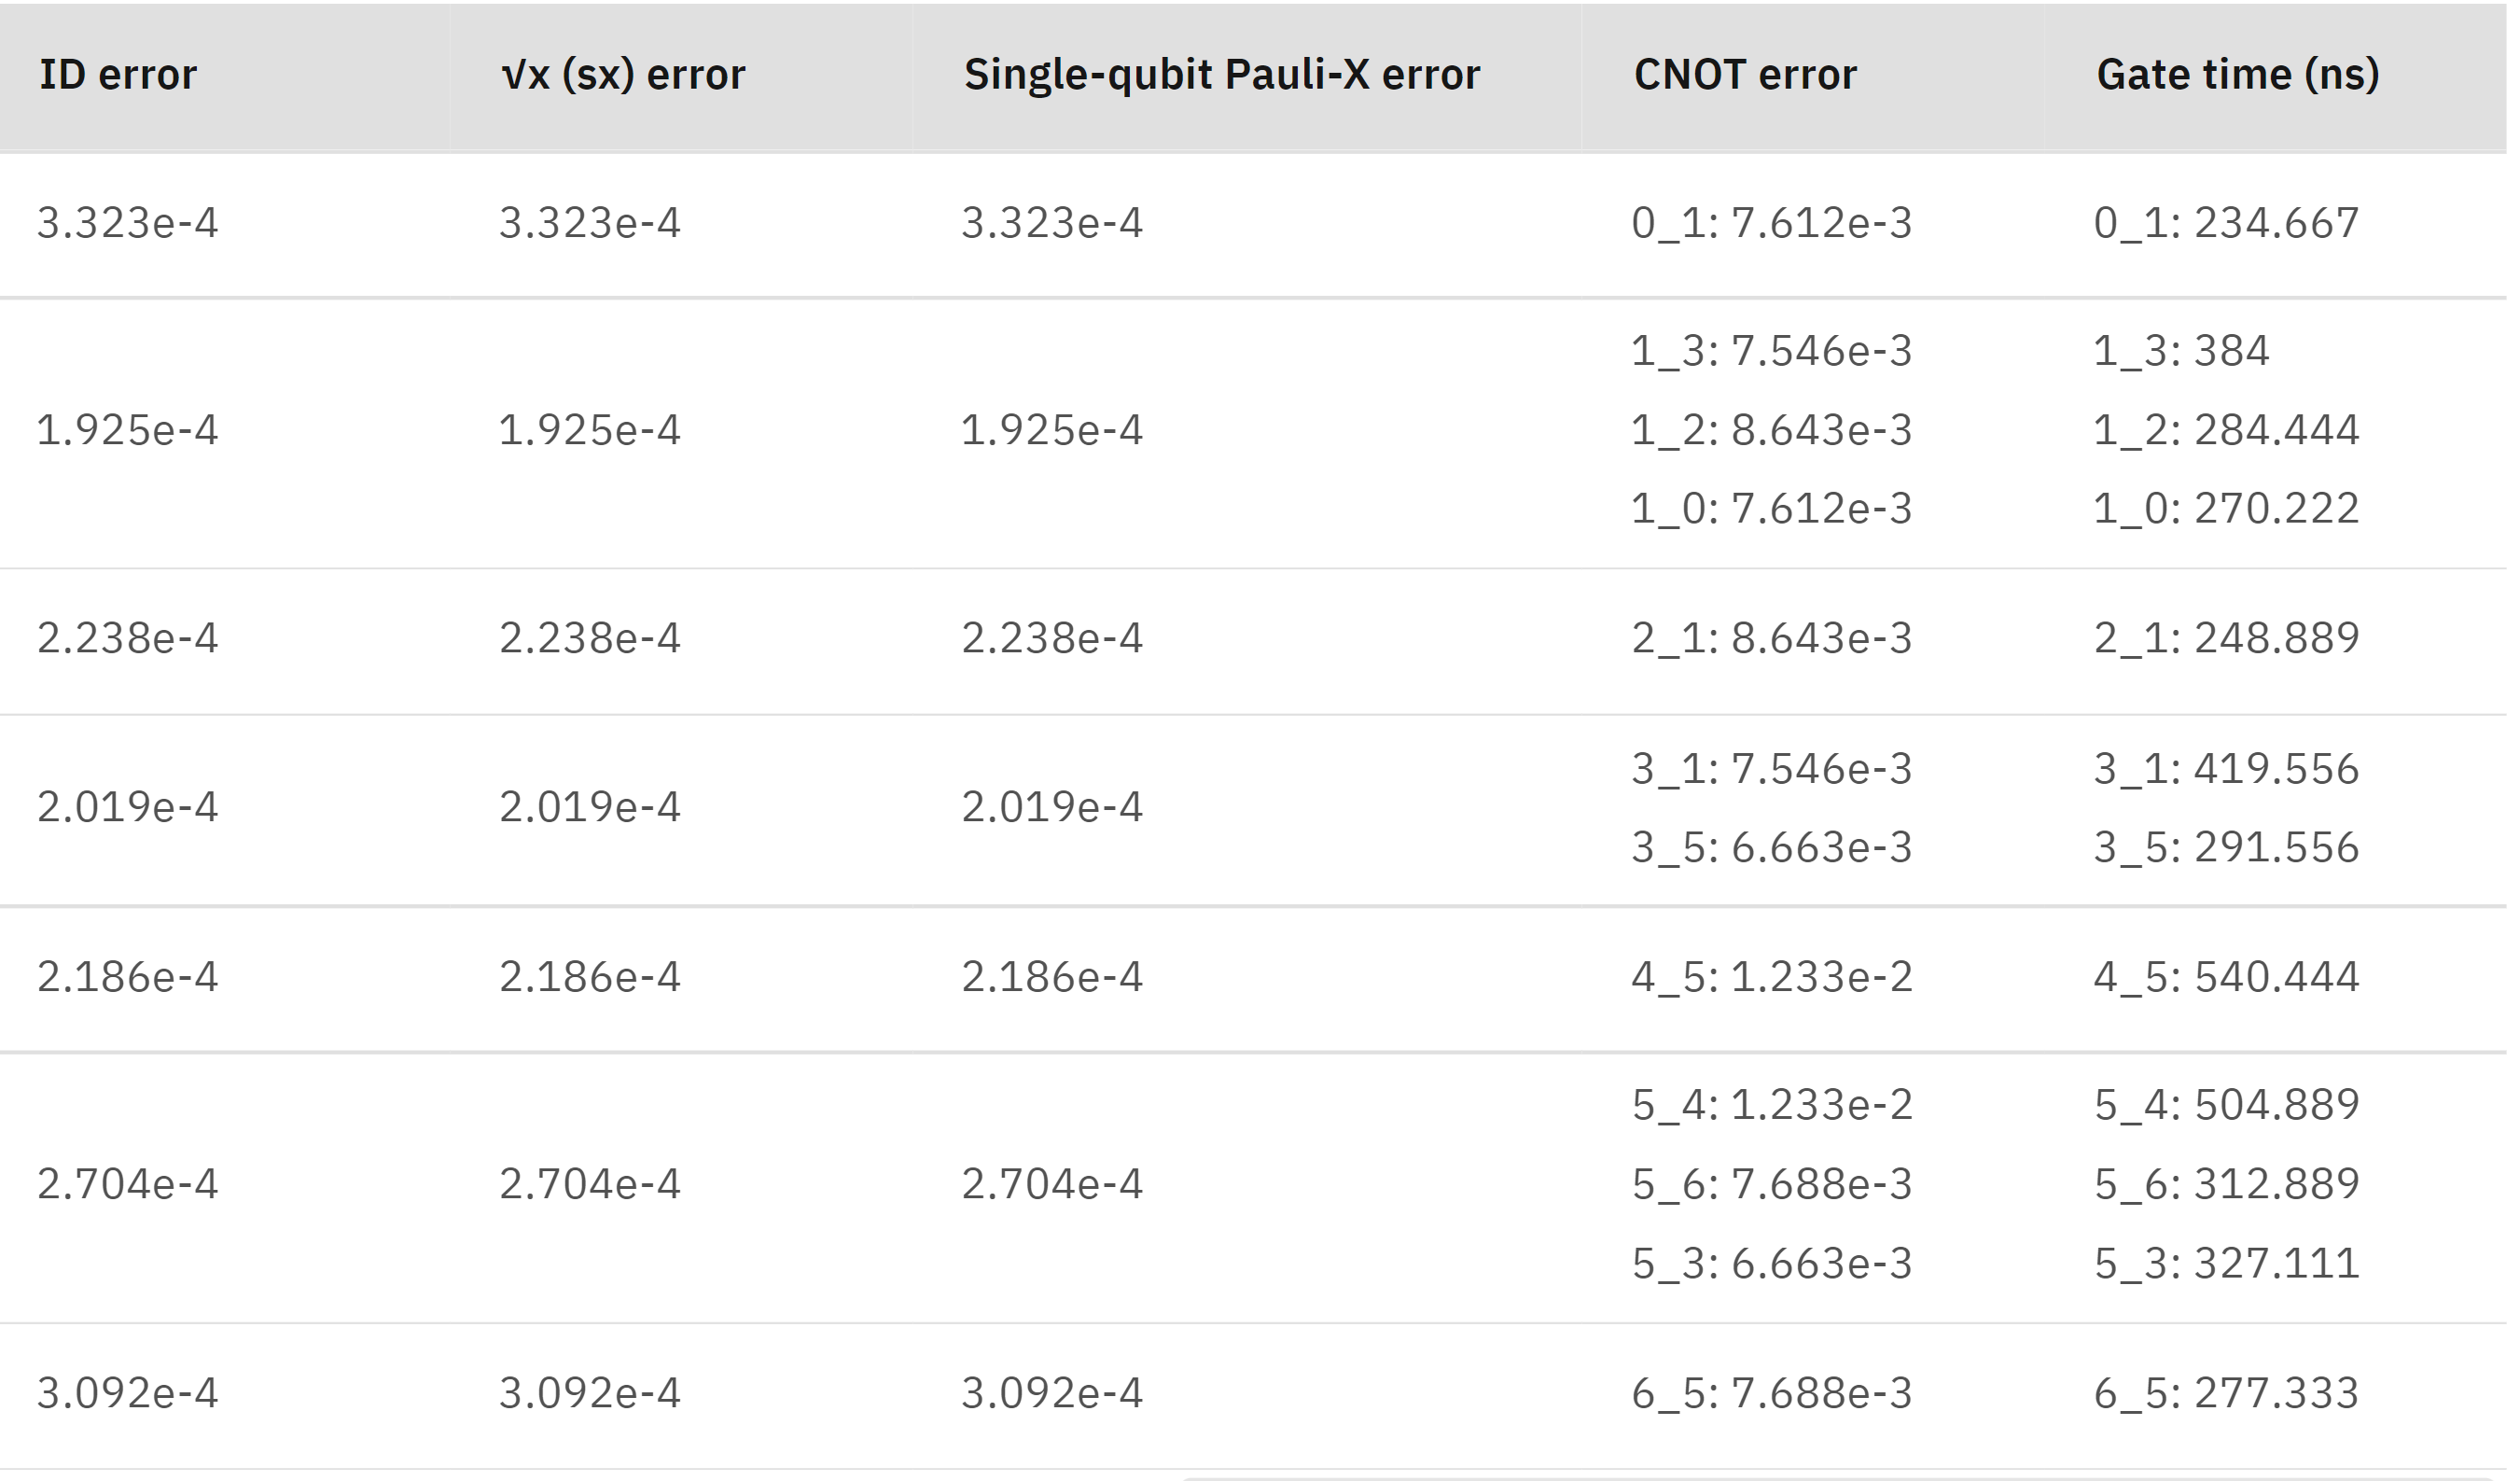
\includegraphics[width = 1.3\textwidth]{jakarta2.png}
\centering
\caption{Gates and errors}
\label{fig:jakarta2}
\end{figure}


\begin{figure}
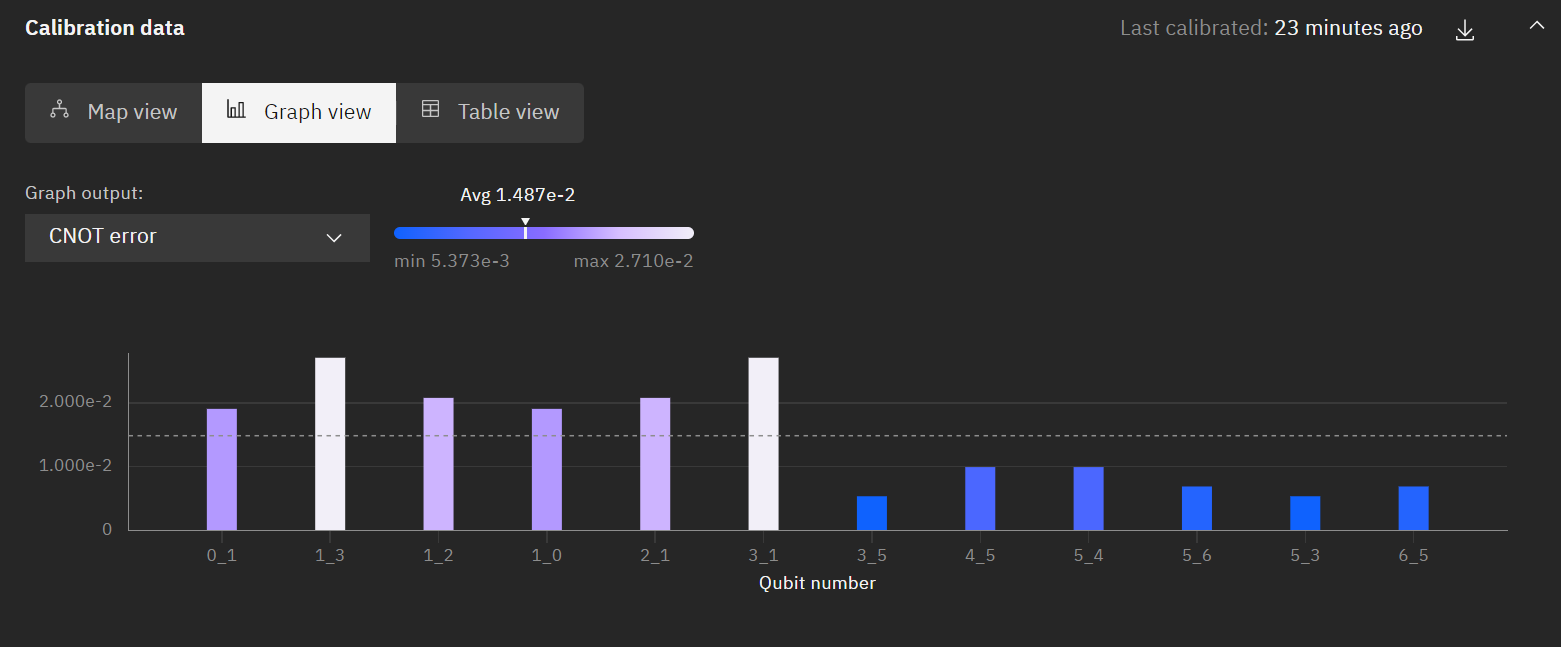
\includegraphics[width = 1.1\textwidth]{error1.png}
\centering
\caption{CNOT errors}
\label{fig:cnot-error}
\end{figure}


\begin{figure}
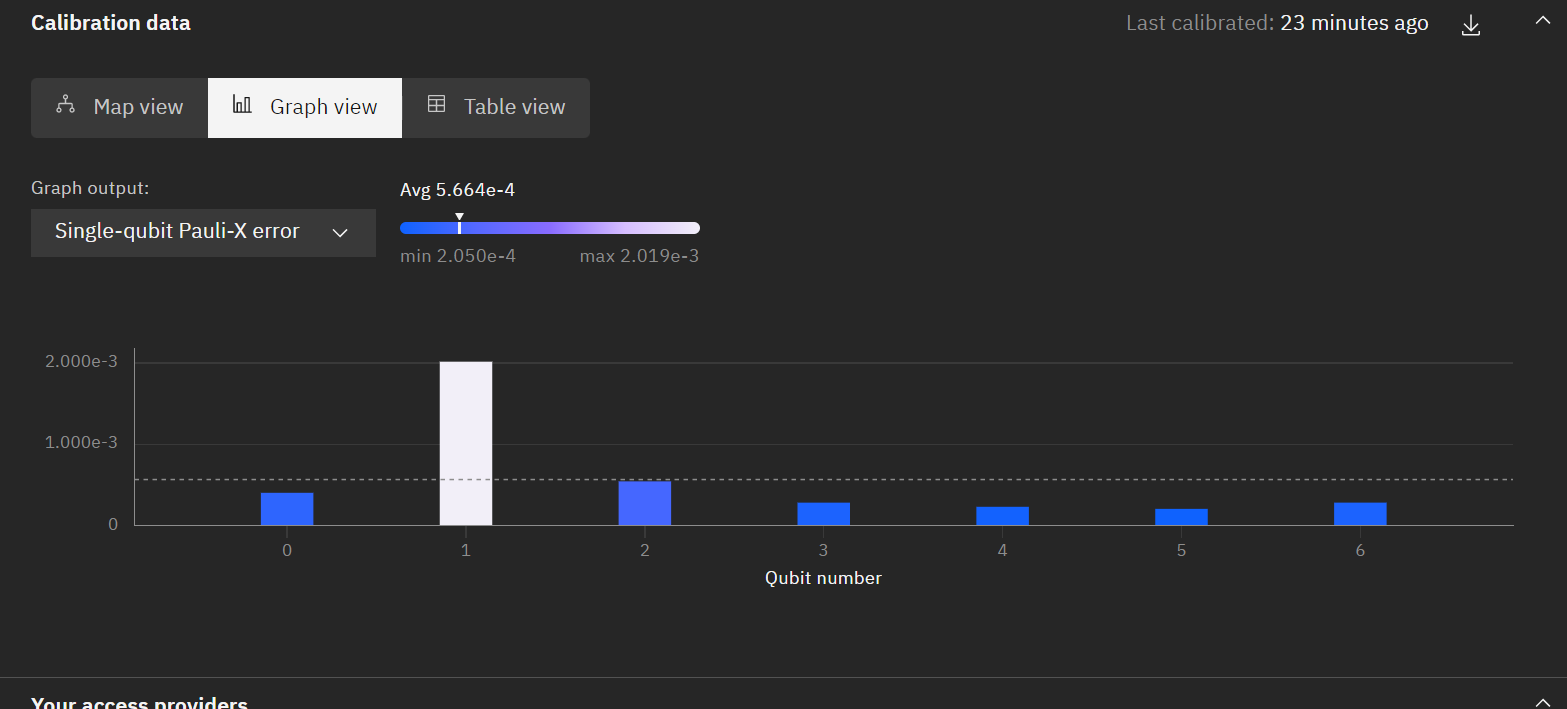
\includegraphics[width = 1.1\textwidth]{error2.png}
\centering
\caption{Single-qubit Pauli-X errors}
\label{fig:pauli-error}
\end{figure}

\begin{figure}
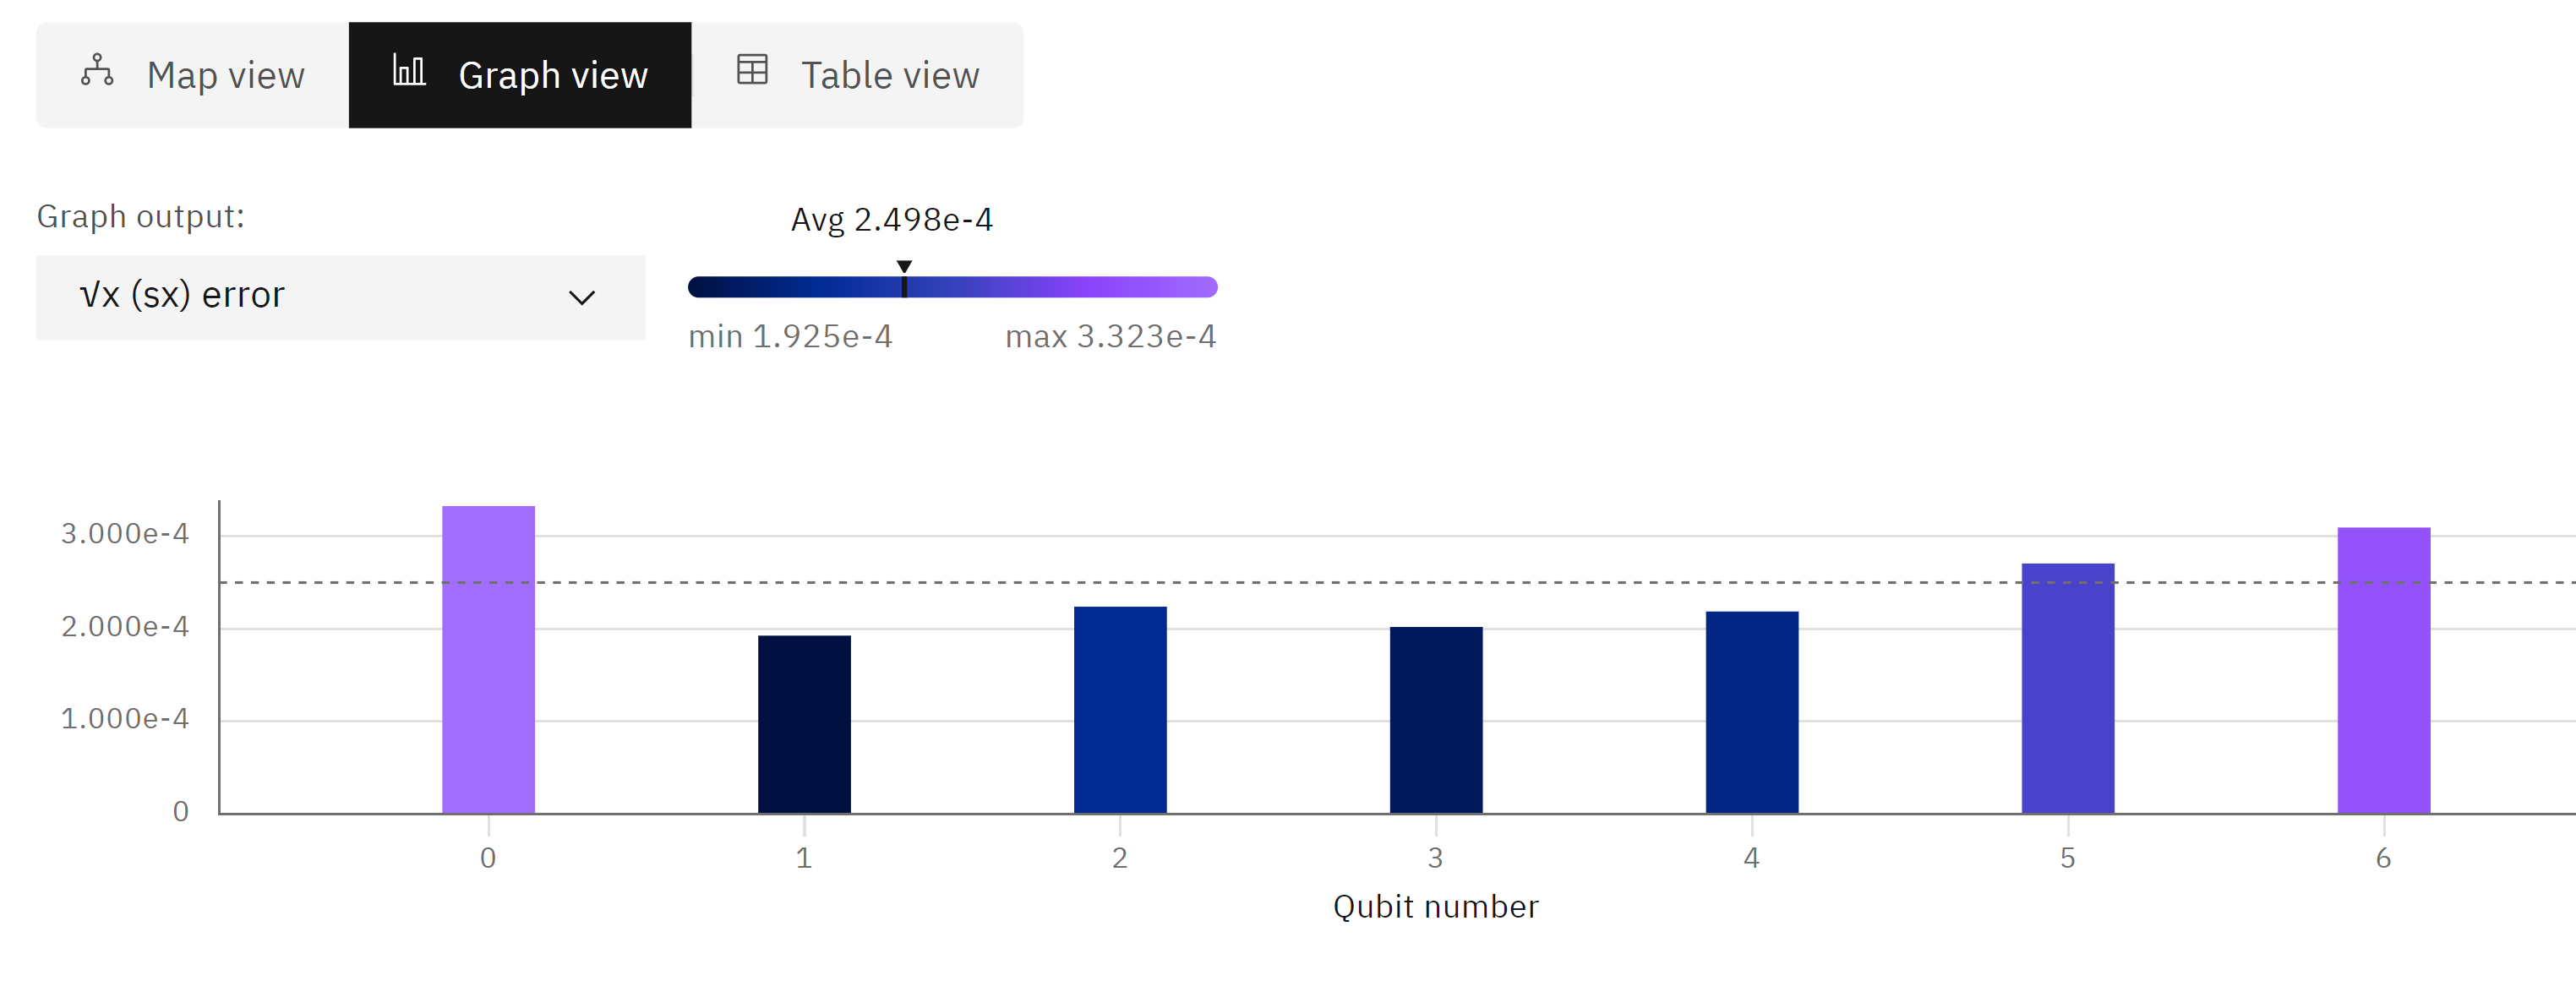
\includegraphics[width = 1.1\textwidth]{error3.png}
\centering
\caption{Sx errors}
\label{fig:sx-error}
\end{figure}
